\chapter{DC Readout}
\label{chapter3}

The initial LIGO detectors used RF heterodyne detection, inspired by
the Pound-Drever-Hall technique, to sense all interferometer length
degrees of freedom and most angular degrees of freedom.  During
Enhanced LIGO, we changed the sensing of the gravitational wave channel (DARM)
to a form of homodyne detection called DC readout.  In
this chapter I explain the motivation for and theory behind DC
readout.

\section{Principle of DC Readout}
A homodyne readout system differs from a heterodyne system by using a
local oscillator at the same (optical) frequency as the field being
measured.  A typical homodyne detection system combines a local
oscillator (LO) field and a signal field via two different ports of a
beamsplitter (depicted in figure~\ref{fig:balanced-homodyne}(a)).  The
two PD signals are subtracted to recover the signal.  This arrangement
suffers from a number of technical
difficulties\cite{McKenzie2007Technical}, including the need to
control the phase of the LO beam, and to maintain the alignment of the
signal and LO beams.

DC readout\footnote{The name `DC readout' probably came about simply
in distinction to `RF readout', with DC (from `direct current') being a
reference to its baseband nature.  It is also
kind of a pun since `direct conversion' is another name for homodyne
detection.} creates the homodyne local oscillator by putting a small
offset into the Michelson or DARM degree of freedom, moving the
interferometer slightly off of the dark fringe.  The resulting carrier
light at the interferometer output port acts as a local oscillator.
This differs from the typical homodyne arrangement in that the two
fields are automatically coincident.  It is no longer necessary to use
two photodiodes, but doing so allows greater power handling capacity,
and allows for the formation of a diagnostic `nullstream'.  The
nullstream is formed from the difference of the two PD signals and
ideally contains only the uncorrelated component of the PD signals.
The sum of the two PD signals provides the intended signal.  The
principle disadvantages of DC readout over the 2-port homodyne
arrangement are that DC readout requires introducing an intentional
microscopic offset of the arms, which can increase noise couplings,
and that DC readout provides little control of the phase of the local
oscillator.

\begin{figure}
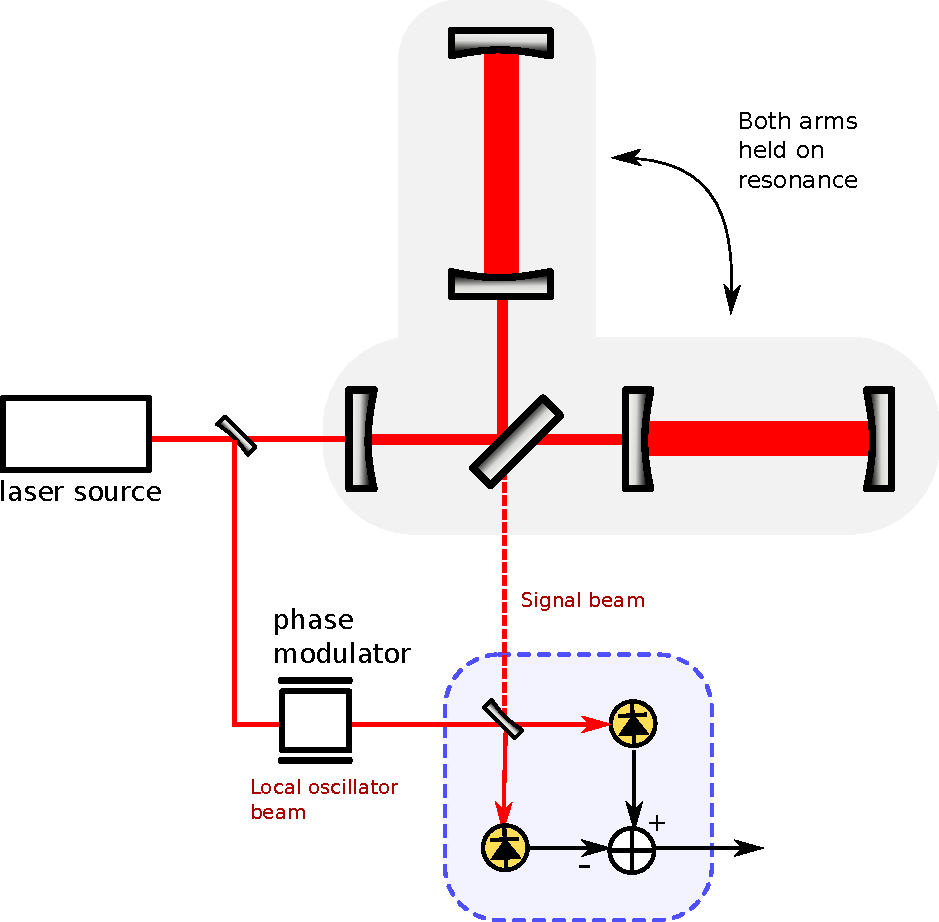
\includegraphics[width=0.5\columnwidth]{figures/homodyne-standard.pdf}
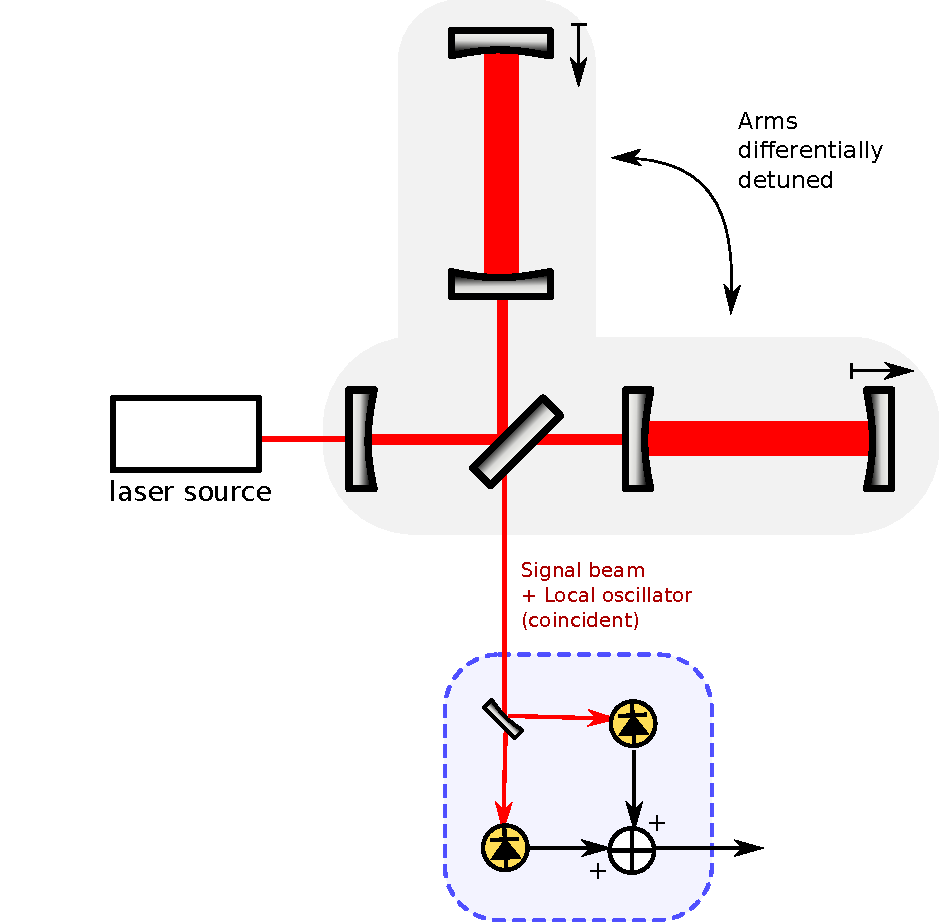
\includegraphics[width=0.5\columnwidth]{figures/homodyne-dc.pdf}
\caption[Comparison of DC readout with balanced homodyne
  detection]{Left: a traditional `balanced photodiode' homodyne
  detection arrangement. Right: DC readout with two photodiodes.
  \label{fig:balanced-homodyne}
}
\end{figure}

\begin{figure}
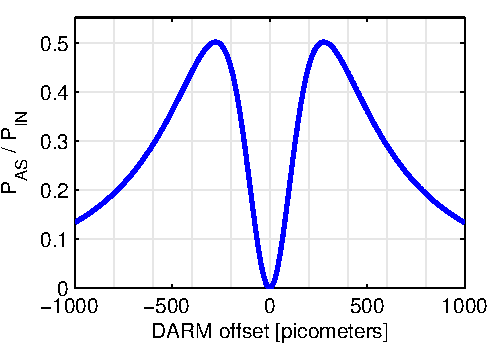
\includegraphics[width=0.5\columnwidth]{figures/darmfringe-1000.pdf}
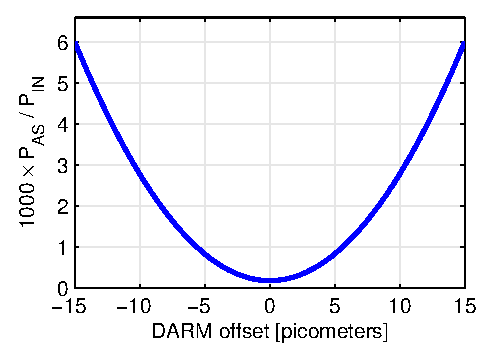
\includegraphics[width=0.5\columnwidth]{figures/darmfringe-15.pdf}
\caption[DARM fringe]{Power at the output port ($P_{AS}$) relative to
  the interferometer input power ($P_{IN}$), as a function of the DARM
  offset, in picometers (1 pm = $10^{-12}$ m).  Left: The DARM fringe
  differs from the $P_{BS} \sin^2 kx$ of a simple Michelson since
  $P_{BS}$ itself depends on the DARM offset.  For comparison recall
  that the full fringe width (from one resonance to the next) is
  $\lambda\approx10^{-6}$ m.  Right: Detail. For small offsets, the
  fringe appears quadratic.  DC readout operates with an intentional
  static DARM offset in order to create a linear relationship between
  DARM perturbations and $P_{AS}$.  The small but nonzero minimum
  power at zero offset is the contrast defect.
  \label{fig:darm-fringe}
}
\end{figure}

One way to intuitively understand DC readout is that simply moving
away from the quadratic point of the fringe (depicted in
figure~\ref{fig:darm-fringe}), a linear relationship from DARM
variations to power variationsis introduced.  On the other hand,
considering the frequency domain picture, we might ask how phase
modulation induced in the arms is converted to amplitude modulation at
the AS port.  The answer is that the Michelson rotates the carrier by
90 degrees due to the $i$ in the Michelson transmission
(equation~\ref{eq:michelson-transmission}).

The true beauty of DC readout is that it exploits the filtering
action of the compound interferometer to produce the local oscillator;
any fluctuations in the amplitude or frequency of the input laser
field are attenuated by the coupled cavity pole before reaching the
output port.

\section{Motivation for DC Readout}

The RF readout technique was used successfully in initial LIGO to
achieve the instruments' design sensitivity.  A number of reasons,
outlined below, motivated the switch to DC readout with an OMC:

\subsubsection*{Improved Noise Couplings} 
The combination of the power recycling cavity and the arm cavities
acts as a single resonant cavity with an effective linewidth of
approximately 1 Hz around the laser carrier.  Intensity and frequency
noise around the laser carrier are reflected from the
interferometer.  The RF sidebands, which are not resonant in the arms,
experience no such filtering in the band of interest.  DC readout
exploits this filtering by using the carrier light that has circulated
in the interferometer as the local oscillator.  The result is that
coupling of noises on the input beam to the gravitational wave readout
can be greatly reduced.

\subsubsection*{Spatial Overlap}  
Imperfect spatial overlap of the signal beam (resonant in the arm
cavities) and the RF sideband beam (resonant in the power recycling
cavity) reduced the optical gain, elevating the shot-noise-limited
noise floor. For instance, a measurement in 2003 found only half the
expected optical gain\cite{Fritschel2003Shot}.  This was alleviated in
part through the use of a thermal compensation system (TCS), which
projected light from a CO$_2$ laser onto optics to adjust their
effective radii of curvature, compensating for thermal lensing.  By
the start of S5 in 2005, no elevation in the shot noise level was
observed\cite{Ballmer2006LIGO}.  However, spurious fields still caused
problems by producing a large signal in the uncontrolled quadrature of
the heterodyne readout (AS\_I); left uncontrolled, this signal would
saturate the photodiode electronics.  This was partially mitigated by
an electronic servo which cancelled this signal in the photodiode
head.

Both DC readout and an OMC mitigate problems with the spatial overlap
of the LO and signal beams.  In DC readout, the local oscillator and
the signal beams are resonate in the same cavities, so spatial overlap
comes naturally.  With either DC or RF readout, an OMC, matched to the
spatial mode of the signal beam, can be used to select the signal beam
and the part of the LO with good spatial overlap.

\subsubsection*{Excess Power}
To cope with the excess power due to higher-order modes at the
interferometer output port, initial LIGO split the light at the
detection port onto four detection photodiodes.  Scaling the
interferometer input power would require a commensurate increase in
the number of photodiodes at the output port and their associated
electronics.  An output mode cleaner reduces the power that needs to
be detected.

\subsubsection*{Homodyne SNR Advantage} 
Homodyne detection confers a fundamental improvement in
signal-to-noise ratio compared to RF readout at shot-noise-limited
frequencies by a factor $\sqrt{3/2}$ (for the same power circulating
in the interferometer).  The extra noise in heterodyne detection is a
result of cyclostationary shot noise\cite{Niebauer1991Nonstationary}
due to the interference between the upper and lower RF sidebands.

\subsubsection*{Squeezed Vacuum Injection} 
Squeezed vacuum injection is an attractive means to decrease the
photon quantum noise in future interferometers by manipulating the
quantum state of the vacuum field that enters the interferometer
through the output port.  Squeezed vacuum injection is more feasible
in conjunction with homodyne detection than with RF readout, since it
requires squeezing in only the audio band rather than at both audio
and RF frequencies\cite{GeaBanacloche1987Squeezed,
  Chelkowski2007Coherent}.  Shot noise reduction via squeezed vacuum
injection has been demonstrated at GEO\cite{GeoSqueezingNature2011}
and an effort is currently underway to implement it at LIGO
Hanford\cite{H1SqueezerProposal}.

\begin{comment}
Some of the motivations of DC readout and an output mode cleaner are:

\begin{itemize}
\item The filtering action of the compound interferometer produces an
  extremely quiet local oscillator.  This reduces the coupling of
  laser noises to the readout.
\item Contributions from noise on the electronic oscillator used to
  create the RF sidebands are greatly reduced.
\item The shot-noise-limited sensitivity of homodyne detection is
  inherently better than that of heterodyne detection, for a fixed
  amount of power on the detection photodiodes, by a factor of at
  least $\sqrt{3/2}$.
\item The shot noise level may be further reduced through the
  injection of squeezed quantum vacuum.  This is much more technically
  feasible with homodyne detection than heterodyne detection.  This
  has recently been demonstrated at the GEO600 detector~\cite{GeoSqueezingNature2011,Vahlbruch2010GEO} and a
  prototype implementation is underway at Hanford~\cite{H1SqueezerProposal}.
\item In DC readout, the signal field and the local oscillator are
  guaranteed to have perfect spatial overlap, since they come from the
  same place.  By contrast, in the conventional heterodyne
  arrangement, the RF fields and the carrier are resonant in different
  cavities and may occupy slightly different spatial modes.  This
  leads to a reduction of shot-noise-limited SNR.  (However, an output
  mode cleaner can be used to force good overlap in either case.)
\item The output mode cleaner greatly decreases the amount of power
  that must be detected by the detection photodiodes by removing
  spurious higher order modes.    
\end{itemize}
\end{comment}

\begin{figure}[p]
\includegraphics{figures/fields-picture.pdf}
\caption[Frequency-domain fields in DC and RF
  readouts]{\label{fig:sideband-picture}Depiction of the fields in DC
  and RF readouts.  (a) In RF readout, the laser carrier is suppressed
  by operating the Michelson on a dark fringe for the carrier.
  Differential phase modulation in the arms becomes amplitude
  modulation of the (suppressed) carrier, depicted as the
  audio-frequency sidebands at $\pm f_{gw}$.  The photodiode sees a
  beat between the GW signal and the RF sidebands.  In homodyne
  readout, a carrier-frequency local oscillator is introduced--in DC
  readout this is done by introducing a microscopic asymmetry between
  the two arms.  The RF sidebands are no longer needed and are removed
  by the output mode cleaner.  The GW-induced sidebands appear as
  amplitude modulation on the carrier, which is sensed directly by the
  photodiodes.}
\end{figure}

\begin{figure}[p]
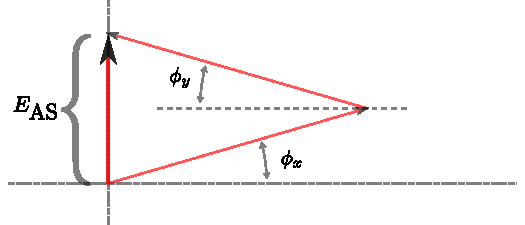
\includegraphics[width=\columnwidth]{figures/phasors.pdf}
\caption[Phasor diagram of DC readout]{\label{fig:mich-phasors}Phasor
  diagram of the fields at the AS port due to the two arms of the
  Michelson.  DARM motion causes equal but opposite rotation of the
  two phasors, which modulates the amplitude of the resultant electric
  field at the AS port ($E_{AS}$).  If this field has a nonzero
  nominal value, as in DC readout, then this will also result in
  linear modulation of $P_{AS}$.}
\end{figure}

\subsection{Calculation of the Optical Gain}

The ratio of signal produced (in Watts) to displacement of DARM (in
meters) is the \emph{optical gain}.  In DC readout, we can find the
optical gain for slow DARM variations by simply taking the derivative
of the power at the anti-symmetric port with respect to changes in
DARM.

From the prior chapter, take the expression for the power at the
output of a Michelson:
\begin{equation}
P_{AS} = P_{BS}\left({r_c}^2 \sin^2 \phi_- + (\Delta r/2)^2 \cos^2 \phi_-\right)
\end{equation}
Taking the derivative with respect to $\phi_-$, we find
\begin{equation}
\frac{d P_{AS}}{d \phi_-} = 2 P_{BS}\left({r_c}^2 - {(\Delta r/2)}^2\right)\cos\phi_- \sin\phi_-
\end{equation}
Immediately we see that any contrast defect ($\Delta r \neq 0$) will diminish the optical gain.  Assuming $r \gg \Delta r$, we can neglect the contrast defect and get simply
\begin{equation}
P_{AS} = P_{BS} {r_c}^2 \sin^2 g_\phi k x
\end{equation}
where $k=2\pi/\lambda$ is the wavenumber, $x$ is the DARM displacement, and $g_\phi$ is the phase gain.
Taking the derivative, we find the optical gain
\begin{align}
S_{DC}  & = \frac{\partial P_{AS}}{\partial x}  \\
       & = 2 P_{BS} {r_c}^2 \sin (g_\phi k x) \cos(g_\phi k x) g_\phi k \\
       & = 2 r_c g_\phi k \sqrt{P_{BS} P_{AS}} \cos(g_\phi k x) \\
       & = 2 {r_c}' k \sqrt{P_{BS} P_{AS}} \cos(g_\phi k x) 
\end{align}
The cosine term is very near unity and can be neglected.  Also, the
phase gain dies off with the cavity pole; and $P_{BS}$ is related to
the input power $P_{IN}$ via the power recycling gain ${g_{cr}}^2$.
Putting this together, we get:
\begin{equation}
\boxed{S_{DC}(f) = 2 g_{cr} {r_c}' k \sqrt{P_{IN} P_{AS}} \left(1 + i\frac{f}{f_c}\right)^{-1}}
\end{equation}

%% To the extent that the introduction of DC offset simply creates a
%% nonzero carrier field at the output port and does not otherwise affect
%% the interferometer dynamics, the frequency response of the interferometer
%% is the same in DC readout as in heterodyne readout, except for an
%% overall scaling. This can be seen by considering the sideband picture
%% (see Figure \ref{fig:sideband-picture}) and is borne out by the following
%% derivation.%

We see that the optical gain scales with the square root of both input
power and the power at the AS port (assuming that the power recycling
gain $g_{cr}$ remains constant, which is approximately true for small
offsets).  From this we can conclude several properties of DC readout
immediately:
%
\begin{itemize}
\item Because the optical gain and the shot noise ASD both scale with
  $\sqrt{P_{AS}}$, the shot-noise-limited sensitivity is insensitive to the
  particular DARM offset we use.
\item The sensitivity of the detector improves with the square root of
  the input power.
\item The frequency response of the interferometer is the same in DC
  readout as in RF readout, up to a scaling factor. (Both are shaped
  simply by the cavity pole.)
\end{itemize}

\section{Selecting the DARM Offset}

The particular DARM offset used to implement DC readout must satisfy a
number of conditions.  On one hand, the DARM offset cannot be too small:
\begin{itemize}
\item The LO field should be of much greater magnitude than the contrast
  defect field, i.e. we must have ${r_c}^2\sin^2\phi_- \gg (\Delta
  r/2)^2 \cos^2\phi_-$, i.e. $\tan \phi_- \gg (\Delta r)/(2r)$.  If this condition is not met, then the SNR
  will suffer from the contrast defect shot noise contribution.
\item The phase offset must be sufficiently large that the response to
  a normal range of DARM motion remains linear.  In particular, the
  DARM offset must be much larger than any expected DARM excursion.
\item The power on the detection photodiode must be large enough such
  that the shot noise exceeds the electronics noise of the readout.
\end{itemize}
On the other hand, there are also upper limits to the magnitude of the
DARM offset, including:
\begin{itemize}
\item The power loss at the AS port must be sufficiently small such
  that the power recycling gain is not diminished excessively.  Excess
  power loss will lead to diminished shot-noise-limited SNR.
\item The power on the detection photodiodes cannot be too high.  Too
  much power on the photodiodes usually produces excess noise or
  reduced quantum efficiency, or will even burn the photodiode.
\item Larger offsets generally increase all of the (laser and
  oscillator) noise couplings and increase the magnitude of optical
  spring effects.  To keep noise couplings small, offsets should
  generally be kept as small as possible.
\item The cavity detuning should be small compared to the cavity pole
  to avoid losing phase gain.  In practice, all of the other criteria
  will become limiting before this one.
\end{itemize}
Several of these criteria are examined in greater detail below.  In
practice, the space of allowed offsets is explored emirically;
colloquially, we turn the knobs in whatever direction makes the noise
go down.  During Enhanced LIGO, we operated with a DARM offset of
approximately 10 picometers.

\begin{figure}[p]
\centerline{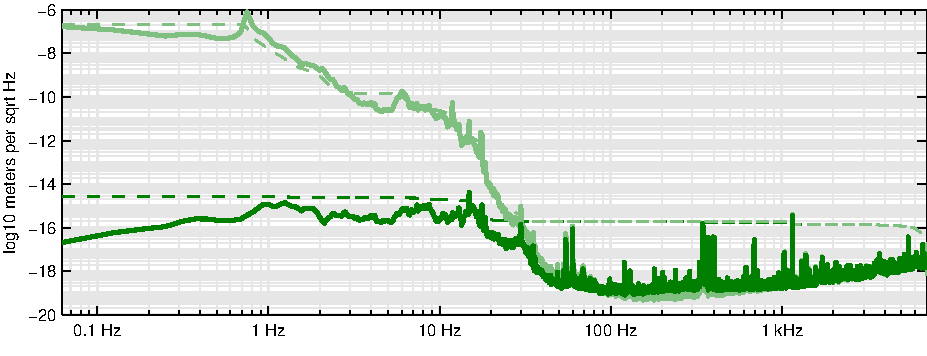
\includegraphics[width=\columnwidth]{figures/residualDARM.pdf}}
\caption[Residual DARM motion]{\label{fig:residual-DARM}DARM
  motion. The lower trace shows the residual motion of DARM after
  stabilization by the DARM control loop.  The upper trace shows the
  `calibrated' DARM, in which the effect of the control loop has been
  removed by multiplying by $(1+G)$, where $G$ is the open loop gain;
  this can be interpreted as `the motion that would be there if there
  were no control loop.'  The control loop reduces the RMS DARM motion
  by ten orders of magnitude in order to hold the interferometer
  within the linear regime around the operating point.  The DARM
  offset used to implement DC readout must be significantly larger
  than the RMS residual motion ($\sim10^{-14}$ m) to avoid
  nonlinear effects.}
\end{figure}


\subsection{Decrease in Arm Power Due to Off-Resonance Operation}
% FIXME: Change this to 'decrease in phase gain...'
The decrease in buildup for a cavity operated off-resonance goes like
$(2\mathcal{F}/\pi)^2\phi^2$, where $\phi$ is the cavity detuning.
For $\mathcal{F}=220$ and $\phi=(2\pi/1064\text{ nm})(10\text{ pm})$,
the fractional power loss is only $7\times10^{-5}$.

\subsection{Decrease in Power Recycling Gain Due to Power Loss at the Output Port}

Allowing power to escape the power recycling cavity (PRC) through the
AS port effectively increases the losses of the PRC, diminishing the
power recycling gain.

The carrier power in the PRC is given by
\begin{equation}
P_{BS} = P_{IN}\left| \frac{t_{RM}}{1 - r_{RM} r_{IFO}}\right|^2
\end{equation}
where $t_{RM}$ is the amplitude transmissivity of the recycling
mirror, $r_{RM}$ is its reflectivity, and $r_{IFO}$ is the amplitude
reflectivity of the rest of the Fabry-Perot Michelson interferometer.
The power-recycling cavity is designed to be critically coupled, so
$r_{IFO}\approx r_{RM}$.

With a DC offset in place, the reflectivity of the Michelson becomes $r_M = r_{IFO}\cos\phi_-$, so we can write
\begin{equation}
P_{BS}(\delta x) \approx P_{IN} 
\frac{T_{RM}}{\left(1 - R_{RM} \cos\left(2\cdot137\cdot k\cdot\delta x\right)\right)^2}
\end{equation}
The loss of power recycling gain becomes significant for large
offsets.  For a 10 pm offset, the reduction in power recycling gain is
only 1\%, but for a 50 pm offset it grows to 20\%.

\subsection{Nonlinearity of the DC Error Signal}

Although we operate sufficiently far from the dark fringe that the
linear coupling of residual DARM motion to output power is dominant,
sufficiently large motion could produce second-order coupling. 

To find the nonlinear contribution, we can expand the power at the AS
port to include the quadratic term, and then we can compare the
quadratic term to the linear term.  Here it is easiest to simply work
in terms of the phase difference at the beamsplitter, $\phi$.
Expanding the fringe around the phase offset $\phi_0$,
%
\begin{equation}
\sin^2\phi \approx \sin^2 \phi_0 
             + 2 (\cos\phi_0 \sin\phi_0) \delta\phi
             + (\cos^2\phi_0-\sin^2\phi_0) (\delta\phi)^2
             + \cdots
\end{equation}
%
where $\delta\phi=\phi-\phi_0$,
we find that the ratio of the quadratic term to the linear term is
%
\begin{equation}
\frac{\cos^2\phi_0-\sin^2\phi_0}{ 2 \cos\phi_0 \sin\phi_0}
\approx
\frac{1}{2}\cot \phi_0 .
\end{equation}
We are interested in the frequency domain contribution of the
quadratic part.  The spectrum of $(\delta\phi(t))^2$ is the
autoconvolution of the spectrum of $\delta\phi(t)$.  In practice, most
of the spectral power in $\delta\phi(t)$ is at very low frequency
(below 1 Hz).  Rather than actually compute the autocorrelation, it
suffices in practice to multiply the amplitude spectral density of
$\delta\phi(t)$ by twice the standard deviation
$\delta\phi_{RMS}=\sqrt{\langle(\delta\phi(t))^2\rangle}$ to estimate
the amplitude spectral density of $(\delta\phi(t))^2$:
\begin{equation}
\delta\phi(f) * \delta\phi(f) \approx 2 \delta\phi_{RMS} \delta\phi(f)
\end{equation}
Using this we can estimate the spectrum of the quadratic contribution as
\begin{equation}
\frac{\text{quadratic}}{\text{linear}} \approx \delta\phi_{RMS} \cot \phi_0 .
\end{equation}
DARM motion of 0.1 pm RMS is equivalent to a $\delta\phi_{RMS}$ of
\begin{align}
\delta\phi_{RMS} &= \delta x_{RMS}  \times g_\phi \times 2\pi / \lambda \\
                &\approx 0.1 \times 10^{-12}\text{ m} \times 137 \times 2\pi / \lambda \\
                &\approx 80  \times 10^{-6} \text{ radians} 
\end{align}
while the static DARM offset of 10 pm becomes
\begin{align}
\phi_0          &\approx 10  \times 10^{-12}\text{ m} \times 137 \times 2\pi / \lambda\\
                &\approx  8  \times 10^{-3} \text{ radians}.
\end{align}
and the ratio of the quadratic contribution to the linear contribution is
\begin{equation}
\frac{\text{quadratic}}{\text{linear}} \approx \delta\phi_{RMS} \cot \phi_0 \approx \frac{\phi_{RMS}}{\phi_0} \approx \frac{1}{1000}.
\end{equation}

The ratio of the quadratic contribution to the linear contribution is
approximately equal to the ratio of the RMS DARM motion to the static
DARM offset.  For a reasonable DARM offset, the quadratic contribution
is a factor of 1000 below the linear contribution.  We would need to
worry about fringe wrapping before the quadratic contribution would
become significant; the nonlinear response of DC readout due to fringe
curvature is negligible.

\begin{comment}
\subsection{DC Readout Elsewhere}
DC readout has been implemented previously at the Caltech 40 meter
prototype \cite{Ward2008DC,RobWardThesis} and the GEO 600
detector\cite{GeoDC,Prijatelj2010,Degallaix2010Commissioning}.  The
current configuration of Virgo incorporates an output mode cleaner but
uses RF heterodyne readout\cite{Acernese2008Virgo}.
\end{comment}

% More references to cite:
% \cite{Adhikari2009DC} % DC readout Normalization for Enhanced LIGO
% \cite{Hild2007Novel} % Crazy detuning
\section{Interferometer Lock Acquisition}

Initial lock acquisition of the Enhanced LIGO interferometers is the
same as in Initial LIGO\cite{Evans2002Lock}. Once the interferometer
is locked using the heterodyne readout schemes, the DARM offset is
introduced to allow carrier light to be transmitted to the output
port. The Output Mode Cleaner is then locked to this carrier
light. Once the OMC is locked to the carrier, control of DARM is
transferred to the DC readout system.  After this transition, a few
other changes are made to engage the OMC alignment servoes and to put
the readout electronics into low noise mode. At this point the
interferometer has reached its operation configuration and
astrophysical data-taking ({}``science mode'') begins.


